% Solution: Tadelis (2013) Exercise 16.4 "School Choice". Input by \solitem.
% Rewritten and deepened from ../pratica-lecture-08-solutions/sol-tadelis-16-4.tex. Check: check_G_L07.py.
\begin{exsol}{Tadelis Exercise 16.4}{336--337}{Exam level}{4}
\asked (a) The extensive form; (b) the matrix of the Bayesian game for $p = \frac12$; (c) all pure-strategy BNE;
(d) all pure-strategy PBE; (e) the intuition for the difference between (c) and (d).

\method Compute payoffs from the table: the student gets the wage minus the learning cost; the firm gets
productivity minus wage in the $H$ job and half the productivity minus wage in the $L$ job. Then the matrix
and its Nash equilibria (= BNE), and the firm's best reply at each of its two information sets for the PBE
(Tadelis \S16.1, pp.~319--323). Slides: Lecture~7, frames~41--44 (Spence: education observed, type not),
45 (separating), 47--48 (pooling and off-path beliefs), 49 (summary). Unlike the slides' Spence model, here
the school \emph{does} change productivity.

\solution
\textbf{Payoffs} (student, firm), with $w_H = 6$, $w_L = 2$:
\begin{center}
\begin{tabular}{llcc}
\toprule
Type & School & Firm assigns $H$ & Firm assigns $L$ \\
\midrule
$E$ & $B$ & $(6 - 2,\ 12 - 6) = (4, 6)$ & $(2 - 2,\ 6 - 2) = (0, 4)$ \\
$E$ & $S$ & $(6 - 0,\ 4 - 6) = (6, -2)$ & $(2 - 0,\ 2 - 2) = (2, 0)$ \\
$G$ & $B$ & $(6 - 8,\ 10 - 6) = (-2, 4)$ & $(2 - 8,\ 5 - 2) = (-6, 3)$ \\
$G$ & $S$ & $(6 - 2,\ 2 - 6) = (4, -4)$ & $(2 - 2,\ 1 - 2) = (0, -1)$ \\
\bottomrule
\end{tabular}
\end{center}

\textbf{(a) Tree.} Nature picks $E$ (probability $p$) or $G$ ($1-p$); the student, knowing his type, picks
$B$ or $S$; the firm sees the school only (one information set after $B$, one after $S$) and assigns $H$ or $L$.
\begin{center}
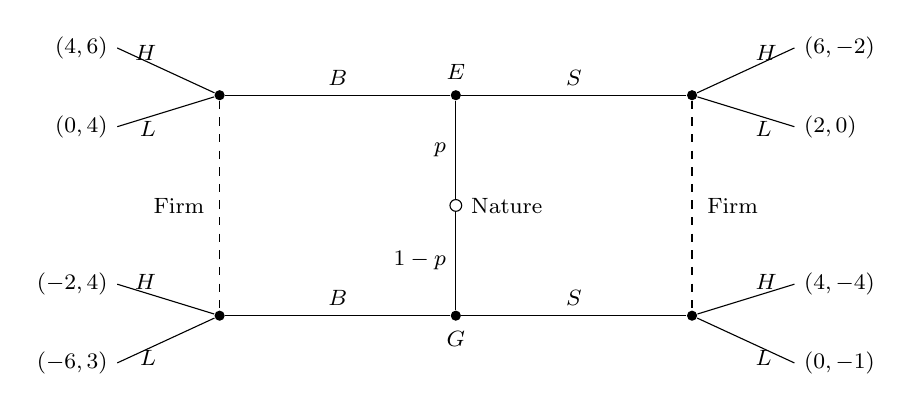
\begin{tikzpicture}[dot/.style={circle,fill,inner sep=1.3pt},every node/.style={font=\footnotesize}]
  \node[circle,draw,inner sep=1.5pt] (n) at (0,0) {};
  \node[right=2pt] at (n) {Nature};
  \node[dot,label=above:{$E$}] (e) at (0,1.4) {};
  \node[dot,label=below:{$G$}] (g) at (0,-1.4) {};
  \draw (e) -- node[left] {$p$} (n) -- node[left] {$1-p$} (g);
  \node[dot] (eb) at (-3,1.4) {}; \node[dot] (gb) at (-3,-1.4) {};
  \node[dot] (es) at (3,1.4) {};  \node[dot] (gs) at (3,-1.4) {};
  \draw (e) -- node[above] {$B$} (eb);  \draw (e) -- node[above] {$S$} (es);
  \draw (g) -- node[above] {$B$} (gb);  \draw (g) -- node[above] {$S$} (gs);
  \draw[dashed] (eb) -- (gb); \draw[dashed] (es) -- (gs);
  \node[left=2pt] at (-3,0) {Firm}; \node[right=2pt] at (3,0) {Firm};
  \draw (eb) -- node[above left] {$H$} ++(-1.3,0.6) node[left] {$(4,6)$};
  \draw (eb) -- node[below left] {$L$} ++(-1.3,-0.4) node[left] {$(0,4)$};
  \draw (gb) -- node[above left] {$H$} ++(-1.3,0.4) node[left] {$(-2,4)$};
  \draw (gb) -- node[below left] {$L$} ++(-1.3,-0.6) node[left] {$(-6,3)$};
  \draw (es) -- node[above right] {$H$} ++(1.3,0.6) node[right] {$(6,-2)$};
  \draw (es) -- node[below right] {$L$} ++(1.3,-0.4) node[right] {$(2,0)$};
  \draw (gs) -- node[above right] {$H$} ++(1.3,0.4) node[right] {$(4,-4)$};
  \draw (gs) -- node[below right] {$L$} ++(1.3,-0.6) node[right] {$(0,-1)$};
\end{tikzpicture}
\end{center}

\textbf{(b) Matrix, $p = \frac12$.} Student: (school of $E$, school of $G$); firm: (job after $B$, job after $S$).
Each cell averages the two types; e.g.\ $(BS, HL)$: $E$ at $B$ in $H$ gives $(4, 6)$, $G$ at $S$ in $L$ gives
$(0, -1)$, so $(2, \frac52)$. Best replies underlined:
\begin{center}
\begin{tabular}{r|c|c|c|c|}
\multicolumn{1}{r}{} & \multicolumn{1}{c}{$HH$} & \multicolumn{1}{c}{$HL$} & \multicolumn{1}{c}{$LH$} & \multicolumn{1}{c}{$LL$} \\ \cline{2-5}
$BB$ & $1,\ \br{5}$ & $1,\ \br{5}$ & $-3,\ \tfrac{7}{2}$ & $-3,\ \tfrac{7}{2}$ \\ \cline{2-5}
$BS$ & $4,\ 1$ & $\br{2},\ \br{\tfrac{5}{2}}$ & $2,\ 0$ & $0,\ \tfrac{3}{2}$ \\ \cline{2-5}
$SB$ & $2,\ 1$ & $0,\ \br{2}$ & $0,\ \tfrac{1}{2}$ & $-2,\ \tfrac{3}{2}$ \\ \cline{2-5}
$SS$ & $\br{5},\ -3$ & $1,\ \br{-\tfrac{1}{2}}$ & $\br{5},\ -3$ & $\br{1},\ \br{-\tfrac{1}{2}}$ \\ \cline{2-5}
\end{tabular}
\end{center}

\textbf{(c) BNE.} Cells with both payoffs underlined: $(BS, HL)$ and $(SS, LL)$.

\textbf{(d) PBE.} At each information set one reply is best \emph{whatever the belief}:
\begin{itemize}
  \item after $B$, $H$ gives $6 > 4$ against $E$ and $4 > 3$ against $G$: $H$ for every belief;
  \item after $S$, $L$ gives $0 > -2$ against $E$ and $-1 > -4$ against $G$: $L$ for every belief.
\end{itemize}
So in every PBE the firm plays $HL$. Then $E$ picks $B$ ($4 > 2$) and $G$ picks $S$ ($0 > -2$). The unique PBE
is the separating profile $(BS, HL)$ with beliefs $\Pr(E \mid B) = 1$ and $\Pr(E \mid S) = 0$, both given by
Bayes' rule. The argument never used $p$, so this holds for every $p \in (0,1)$. $(SS, LL)$ is not a PBE: it
needs $L$ after $B$, which no belief supports.

\textbf{(e) Intuition.} In $(SS, LL)$ nobody goes to Brown Bear, so the firm's plan after $B$ is never tested: the
BNE lets it ``threaten'' to waste a Brown Bear graduate in the low-tech job, which deters the excellent type from
signaling. PBE asks the firm to be sequentially rational at every information set, on or off the path, and
$H$ after $B$ is optimal for every belief, so the threat falls and the excellent type separates.

\interp School choice works as a signal because it is relatively cheaper for the excellent type: $B$ costs $E$ two
more than $S$, but costs $G$ six more, and the $H$ job's premium of $4$ lies between ($2 \le 4 \le 6$) --- the
slides' condition $c_H \le w \le c_L$ (frame~45) in increments. Here Brown Bear also raises productivity, so
part of the separation is efficient, not only a signal.

\verify \texttt{check\_G\_L07.py} recomputes the eight payoff pairs from wages, costs and productivities, finds
the BNE $(BS, HL)$ and $(SS, LL)$ at $p = \frac12$, and confirms that $(BS, HL)$ is the only pure PBE for
$p \in \{\frac1{20}, \dots, \frac{19}{20}\}$ and that $H$ (after $B$) and $L$ (after $S$) are dominant at their sets.
Output: ``Tadelis 16.4: p = 1/2 BNE (BS,HL), (SS,LL); unique PBE (BS,HL) for every p (H dominant after B, L
dominant after S)''. Tadelis prints no answer.

\mistakes
\begin{itemize}
  \item Paying the firm the full productivity in the $L$ job. The table says half: e.g.\ $E$ from Brown Bear in
  $L$ yields $\frac{12}{2} - 2 = 4$, not $10$.
  \item Subtracting the learning cost from the firm's payoff. The cost falls on the student only.
  \item Looking for a pooling PBE on $S$ by choosing a pessimistic belief after $B$. No belief helps: $H$ after $B$
  is dominant, so the off-path belief is irrelevant here.
  \item Writing the firm's strategy as one action: it is a pair (job after $B$, job after $S$).
\end{itemize}

\answer{(b) Matrix above. (c) BNE: $(BS, HL)$ and $(SS, LL)$. (d) Unique PBE: $(BS, HL)$ --- the excellent type
goes to Brown Bear, the good type to Silly Tree, the firm assigns $H$ after $B$ and $L$ after $S$, beliefs
$\Pr(E \mid B) = 1$, $\Pr(E \mid S) = 0$, for every $p$. (e) $(SS, LL)$ rests on a non-credible reply to the
unused message $B$; sequential rationality removes it.}
\end{exsol}
